\chapter{Model}
\label{chp:model}
In this chapter, we will define the type of image-based recommendation system that we used as the foundation for our subsequent robustness studies. More specifically, we will provide a detailed description and evaluation of our adopted two-stage model, based on the work of \cite{tuinhof2018image}.

\section{Image-Based Recommendation System}
We chose to reproduce the model, published by \cite{tuinhof2018image}, for our following experiments, as it relies purely on content-based data and utilizes the publicly available DeepFashion dataset. The proposed approach consists of two stages: a \ac{CNN} fashion classifier, predicting category and texture of garments, and a similarity search using a \ac{k-NN} algorithm, based on the computed latent space feature embeddings from the classifier. This rather simple technique proves successful at finding similar items based on the texture and category of a supplied input image. 

Due to a non-disclosure agreement, signed by the authors of the original paper, it was unfortunately not possible to retrieve their source code or model weights. Therefore, we had to reproduce the results from scratch. In the following subsections, we will document our reproduced results, and describe some minor improvements.

\subsection{Convolutional Deep Fashion Classifier}
\label{sec:fashion-classifier}
In the first step, we train a \ac{CNN} to predict the category and texture type of fashion garments simultaneously. The authors of the original paper trained two individual networks for each task and concatenated both networks' embeddings for the second-stage \ac{k-NN} search. Since studies have shown that multi-task learning can lead to significant performance improvements \parencite{zhang2017survey}, we decided to evaluate training a network on both tasks at once, using two independent fully connected softmax layers, instead of one, as a prediction head. Formally, our multi-task model can be written as
\begin{equation}
\mathcal{N}(\mathbb{W}, \boldsymbol{X}) = [\mathcal{S}(\mathbb{C}, \mathcal{F}(\mathbb{I}, \boldsymbol{X})),\,\mathcal{S}(\mathbb{T}, \mathcal{F}(\mathbb{I}, \boldsymbol{X}))],
\label{eq:fashion-cnn}
\end{equation}
where $\mathbb{W} = (\mathbb{I},\mathbb{C},\mathbb{T})$ are weight matrices, $\mathcal{S}(\mathbb{C},\boldsymbol{X})$ and $\mathcal{S}(\mathbb{T},\boldsymbol{X})$ are fully connected softmax output layers that perform the classifications for category and texture, and $\mathcal{F}(\mathbb{I}, \boldsymbol{X})$ is the shared \ac{CNN} backbone, which is used as a feature extractor.

The original paper evaluated two state-of-the-art \ac{CNN} architectures at the time of publication-- Inception with batch norm and AlexNet. Since then, many more efficient architectures, like ShuffleNet \parencite{ma2018shufflenet} and MobileNetV2 \parencite{sandler2018mobilenetv2}, have been proposed. Due to its superior performance, we chose to use MobileNetV2 as our architecture for the \ac{CNN} backbone. As an initialization for the weights, we used the weights of a pre-trained network on ImageNet\,\footnote{Pre-Trained MobileNetV2 \url{https://pytorch.org/hub/pytorch_vision_mobilenet_v2/}}. This way of initializing networks is called transfer learning and has proven to be beneficial for convergence \parencite{shin2016deep}. For training the MobileNetV2, we use the Adam \parencite{Kingma:2014} optimizer with a batch size of 32, and a learning rate of 0.001. Our training history can be seen in Figure~\ref{fig:classifier-tensorboard} and our final evaluation results on the test set in Table~\ref{tab:classifier-results}

\begin{figure}[H]
	\centering
	\subfloat[][Plot of combined model loss on training and test dataset]{
		\resizebox{0.45\textwidth}{!}{\begin{tikzpicture}
\begin{axis}[
axis background/.style={fill=color0},
axis line style={white},
legend cell align={left},
legend style={fill opacity=0.8, draw opacity=1, text opacity=1, at={(0.03,0.97)}, anchor=north west, draw=none, fill=color0, font=\scriptsize},
tick align=outside,
tick pos=left,
x grid style={white},
xmajorgrids,
xtick style={color=white!15!black},
scaled y ticks = false, 
scaled x ticks = false, 
y grid style={white},
ymajorgrids,
ytick style={color=white!15!black},
ticklabel style = {font=\scriptsize},
xlabel=$step$, ylabel={$loss$}
]
\addplot [ultra thick, color1, smooth] table [x=Step, y=Value, col sep=comma] {images/tensorboard/loss-train.csv};
\addlegendentry{train}
\addplot [ultra thick, color3, smooth] table [x=Step, y=Value, col sep=comma] {images/tensorboard/loss-test.csv};
\addlegendentry{test}
\end{axis}
\end{tikzpicture}}
	}\hspace{0.5cm}
	\subfloat[][Plot of category accuracy on training and test dataset]{
		\resizebox{0.45\textwidth}{!}{\begin{tikzpicture}
\begin{axis}[
axis background/.style={fill=color0},
axis line style={white},
legend cell align={left},
legend style={fill opacity=0.8, draw opacity=1, text opacity=1, at={(0.03,0.97)}, anchor=north west, draw=none, fill=color0, font=\scriptsize},
tick align=outside,
tick pos=left,
x grid style={white},
xmajorgrids,
xtick style={color=white!15!black},
scaled y ticks = false, 
scaled x ticks = false, 
y grid style={white},
ymajorgrids,
ytick style={color=white!15!black},
ticklabel style = {font=\scriptsize},
xlabel=$step$, ylabel={$accuracy$}
]
\addplot [ultra thick, color1, smooth] table [x=Step, y=Value, col sep=comma] {images/tensorboard/accuracy-train.csv};
\addlegendentry{train}
\addplot [ultra thick, color3, smooth] table [x=Step, y=Value, col sep=comma] {images/tensorboard/accuracy-test.csv};
\addlegendentry{test}
\end{axis}

\end{tikzpicture}}
	}\\
	\subfloat[][Plot of category classification loss on training dataset]{
		\resizebox{0.45\textwidth}{!}{\begin{tikzpicture}
\begin{axis}[
axis background/.style={fill=color0},
axis line style={white},
legend cell align={left},
legend style={fill opacity=0.8, draw opacity=1, text opacity=1, at={(0.03,0.97)}, anchor=north west, draw=none, fill=color0, font=\scriptsize},
tick align=outside,
tick pos=left,
x grid style={white},
xmajorgrids,
xtick style={color=white!15!black},
scaled y ticks = false, 
scaled x ticks = false, 
y grid style={white},
ymajorgrids,
ytick style={color=white!15!black},
ticklabel style = {font=\scriptsize},
xlabel=$step$, ylabel={$loss$}
]
\addplot [ultra thick, color1, smooth, each nth point=8] table [x=Step, y=Value, col sep=comma] {images/tensorboard/loss-category.csv};
\addlegendentry{train}
\end{axis}
\end{tikzpicture}
}
	}\hspace{0.5cm}
	\subfloat[][Plot of texture classification loss on training dataset]{
		\resizebox{0.45\textwidth}{!}{\begin{tikzpicture}
\begin{axis}[
axis background/.style={fill=color0},
axis line style={white},
legend cell align={left},
legend style={fill opacity=0.8, draw opacity=1, text opacity=1, at={(0.03,0.97)}, anchor=north west, draw=none, fill=color0, font=\scriptsize},
tick align=outside,
tick pos=left,
x grid style={white},
xmajorgrids,
xtick style={color=white!15!black},
scaled y ticks = false, 
scaled x ticks = false, 
yticklabel style={
	/pgf/number format/fixed,
	/pgf/number format/precision=5
},
y grid style={white},
ymajorgrids,
ytick style={color=white!15!black},
ticklabel style = {font=\scriptsize},
xlabel=$step$, ylabel={$loss$}
]
\addplot [ultra thick, color1, smooth, each nth point=8] table [x=Step, y=Value, col sep=comma] {images/tensorboard/loss-texture.csv};
\addlegendentry{train}
\end{axis}
\end{tikzpicture}
}
	}
	\caption{Training history of our fashion classifier trained for 24 epochs}
	\label{fig:classifier-tensorboard}
\end{figure}
\pagebreak

\begin{table}[H]
	\centering
\subfloat[][Our category classifier results in comparison to the results reported in the original paper by \cite{tuinhof2018image}.]{
		\label{tab:category-results}
\begin{tabular}{ lcc } 
		\toprule		
		Category        & Ours & \cite{tuinhof2018image} \\
		\midrule
		Accuracy	    & 68.25 & 63.00\\
		Top-5 Accuracy  & 93.14 & 84.00 \\
		CE-Loss         & 1.09  & 1.27 \\
		\bottomrule
\end{tabular}
}
\hfill
\subfloat[][Our texture classifier results.]{
	\label{tab:texture-results}
\begin{tabular}{ lcc } 
	\toprule		
	Texture          & Ours  \\
	\midrule
	Top-1 Precision  & 43.68\\
	BCE-Loss         & 0.03  \\
	\bottomrule
\end{tabular}
}
\caption{Evaluation results on test set for our multi-task \textit{DeepFashion} classifier.}
\label{tab:classifier-results}
\end{table}

As seen in Table~\ref{tab:category-results}, we slightly outperform the original accuracy metric on the category classification task by about 5\%. The authors of the DeepFashion dataset formulated the second task of texture classification as a multi-label problem. \cite{tuinhof2018image}, on the other hand, chose to reformulate it as a single label task, by randomly sampling one label from the set of correct labels. We chose to treat the texture label as a multi-label task and make use of the entire dataset. Therefore, our results for the texture classifier are not directly comparable to \cite{tuinhof2018image}, as the metrics and losses used in single and multi-label settings differ. As a loss function for the texture classifier, we used the \ac{BCE} function, which performs elementwise sigmoid activations instead of a softmax activation, as in the case of categorical \ac{CE}. Our results in Table~\ref{tab:texture-results} show that our network has been reasonably successful at learning the task of texture classification, achieving almost 44\% precision on the top predicted texture from 156 possible classes. We also applied several standard image augmentation techniques to increase the dataset size effectively and prevent overfitting. These include random rotations with a maximum rotation angle of $\pm15\degree$, random rescaling, and cropping within a range of [75\%, 125\%] and random horizontal flips.

\subsection{Ranking in Feature Space using k-NN Search}
The \ac{CNN} backbone is used as a feature extractor, and returns feature vectors $\mathcal{F}(\boldsymbol{X})$ of size $d= 1280$ for any input image. This feature extractor is applied to all $n= 106,649$ images from the dataset, as described in Chapter~\ref{chp:dataset}. The resulting vectors are stacked to obtain a $n\times d$ article embedding matrix, which we use for a k-NN ranking algorithm.

\begin{align}
sim(A, B) &= \frac{\mathbf{A} \cdot \mathbf{B}}{\|\mathbf{A}\| \|\mathbf{B}\|}
\label{eq:sim}\\
dist(A, B) &= 1 - sim(A,B)
\label{eq:dist}
\end{align}
 
As a similarity measure, we use the cosine distance, defined in Equation~\ref{eq:dist}, which is commonly used in recommendation systems \parencite{desrosiers2011comprehensive}. To improve the performance of the \ac{k-NN} search, we additionally use an approximate nearest neighbor index\footnote{NMSLIB \url{https://github.com/nmslib/nmslib}}, that uses a highly optimized data structure, called \ac{HNSW} graphs, which was originally published by \cite{malkov2018efficient}.

The resulting embedding space of articles is visualized in Figure~\ref{fig:tsne}. Similar categories and textures are grouped due to their proximity in feature space, which indicates the usefulness of our generated embeddings for finding similar articles. The ranked nearest neighbors for two randomly chosen articles can be seen in Figure~\ref{fig:reco}. Subjectively, the recommendations indeed look quite similar to the query images.

\begin{figure}
	\centering
	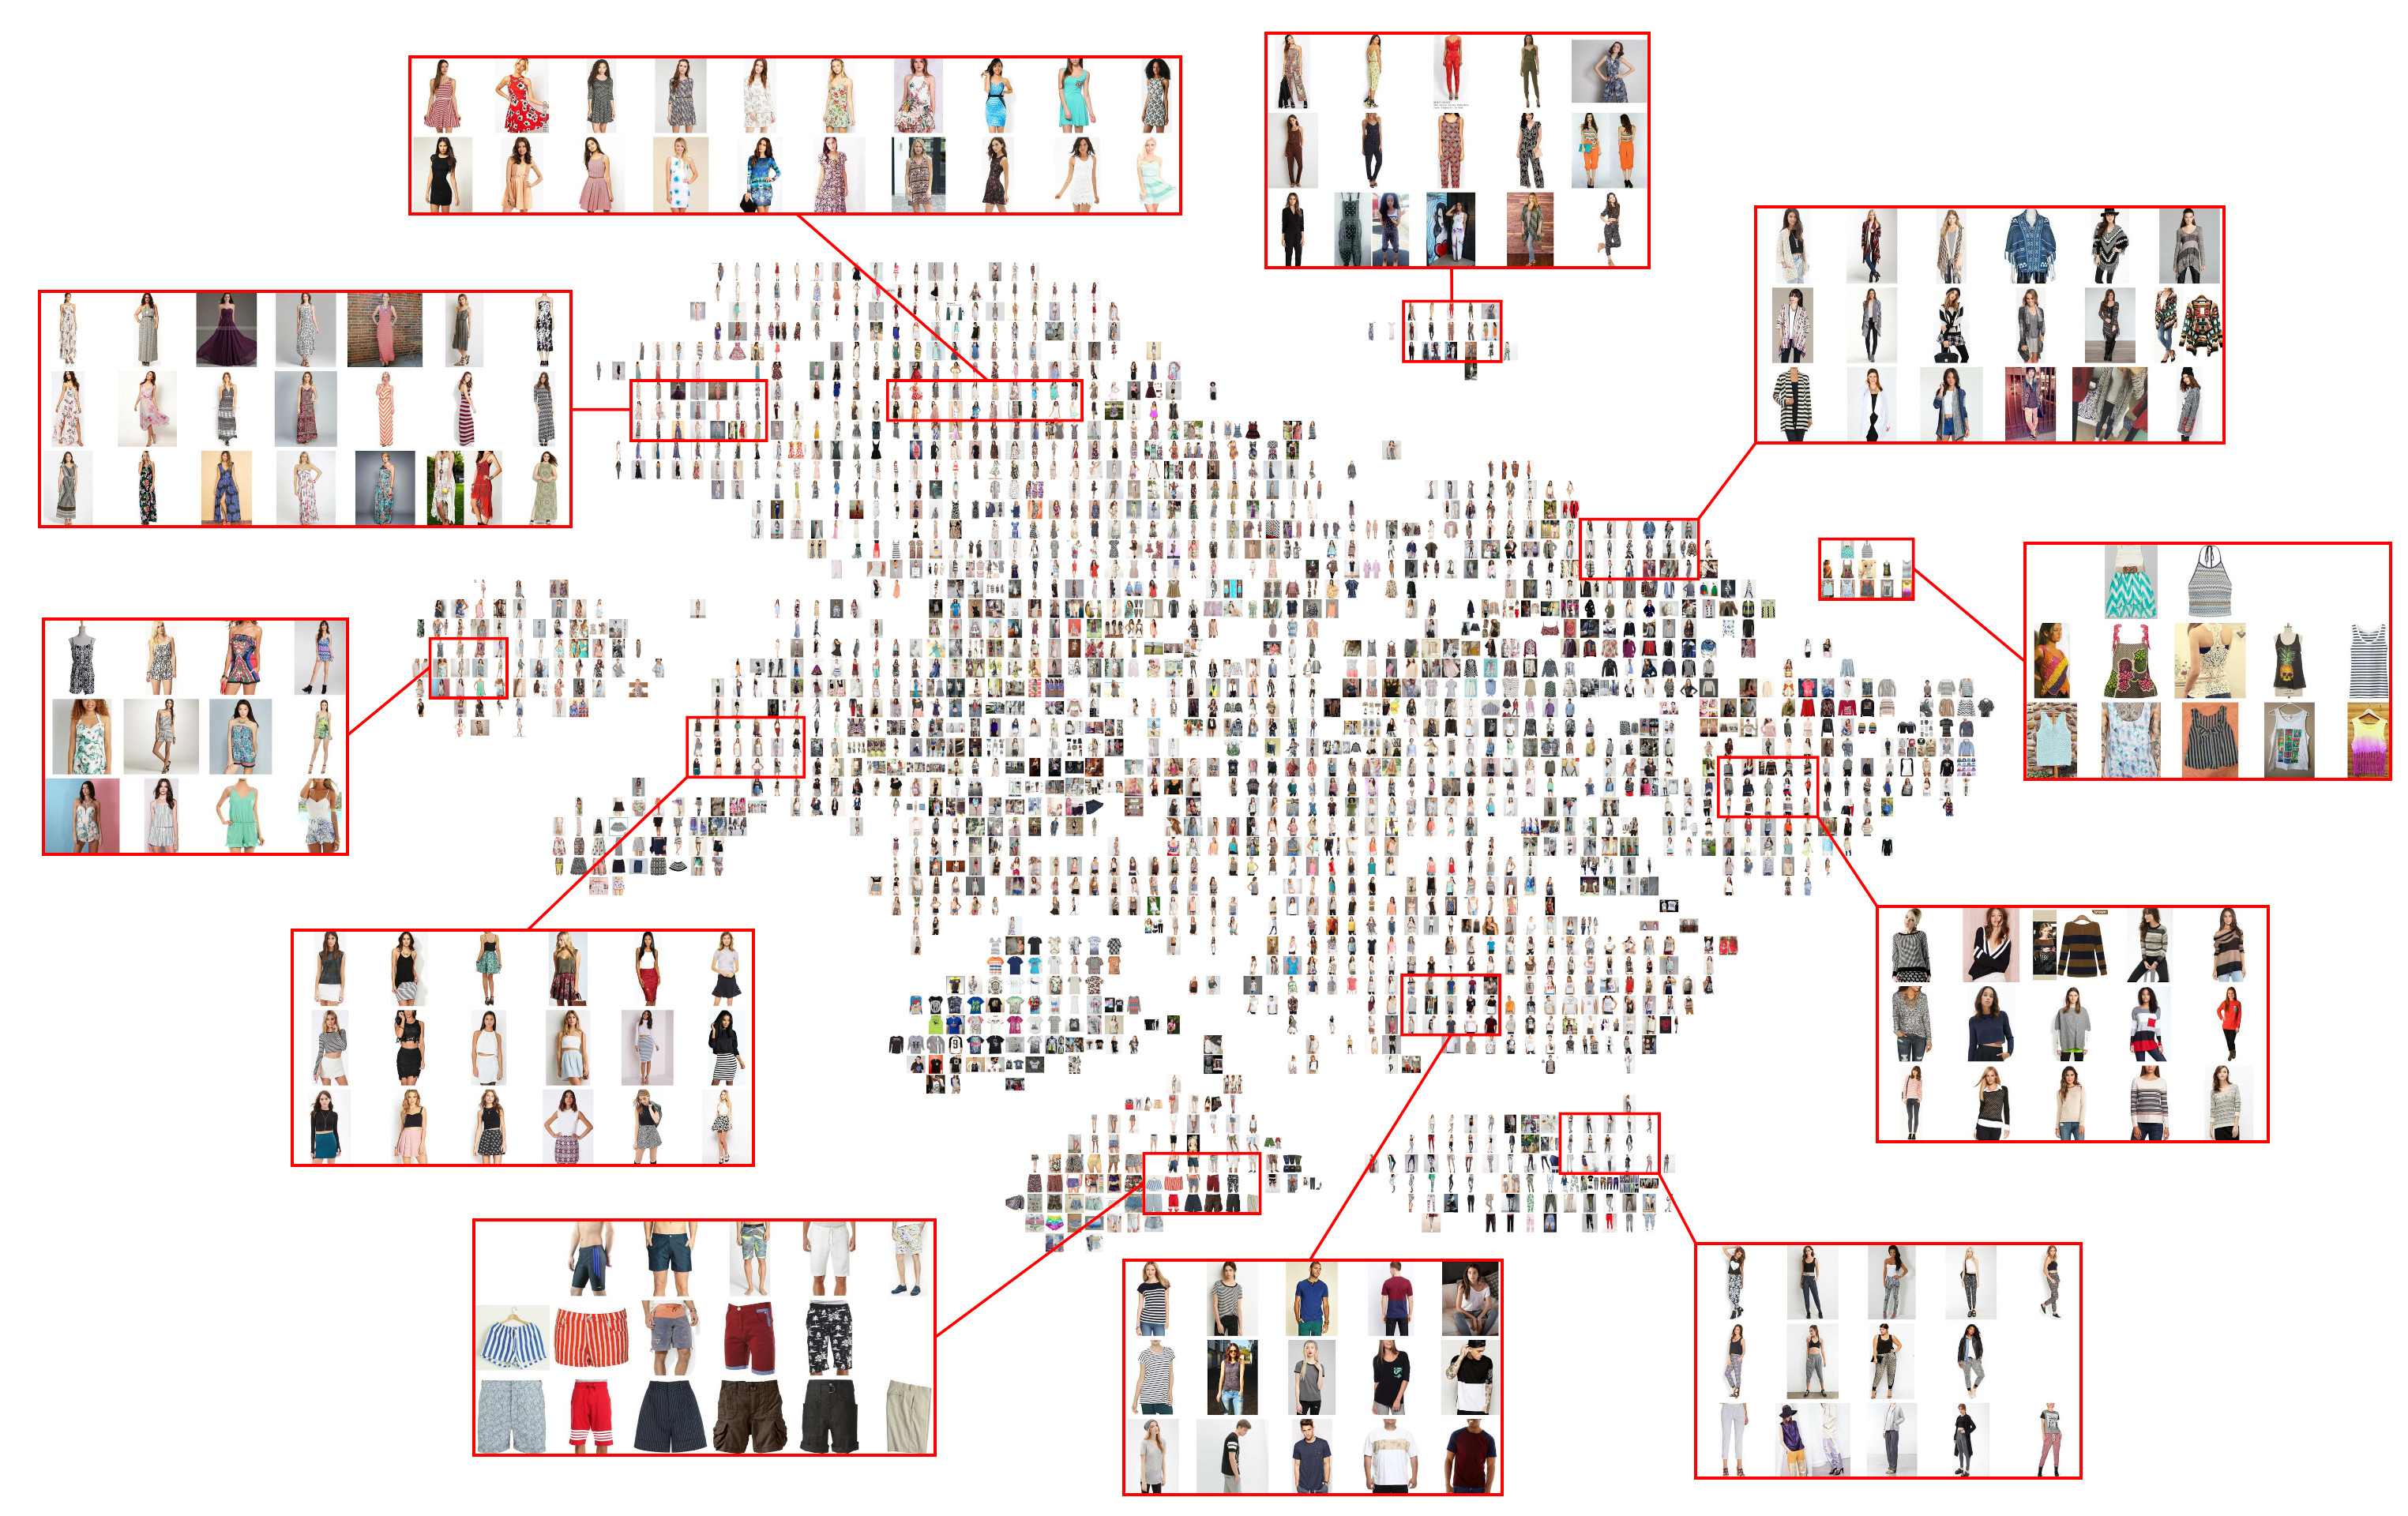
\includegraphics[width=\textwidth]{images/tsne/normal-24-epochs-magnified-rescaled}
	\caption{\acs{t-SNE} visualization of articles from the DeepFashion dataset, using their feature vectors from the penultimate layer of the classifier trained in Section \ref{sec:fashion-classifier}. For clarity, the space is discretized into a grid and for each grid cell one image is randomly selected among overlapping instances.}
	\label{fig:tsne}
\end{figure}

\begin{figure}[H]
	\centering
	\begin{tikzpicture}

\node [rectangle, inner sep=0.5pt, color1, draw, thick] (query1) {\includegraphics[width=2.25cm] {../../data/DeepFashion/img_resized/Stripe_V-Neck_Tee/img_00000080.jpg}};
\node [above=of query1, yshift=-1cm, color1, font=\small] {\textbf{Query} image};


\node [right=of query1, rectangle, inner sep=0.5pt, color2, draw, thick] (orig1) {\includegraphics[width=2cm] {../../data/DeepFashion/img_resized/Classic_Striped_Tee/img_00000055.jpg}};
\node [above=of orig1, yshift=-1cm, color2, font=\small] {$dist = 0.0141$};

\node [right=0.5cm of orig1, rectangle, inner sep=0.5pt, color2, draw, thick] (orig2) {\includegraphics[width=2cm] {../../data/DeepFashion/img_resized/Micro-Stripe_Pocket_Tee/img_00000017.jpg}};
\node [above=of orig2, yshift=-1cm, color2, font=\small] {$dist = 0.0181$};

\node [right=0.5cm of orig2, rectangle, inner sep=0.5pt, color2, draw, thick] (orig3) {\includegraphics[width=2cm] {../../data/DeepFashion/img_resized/Striped_Crew_Neck_Tee/img_00000017.jpg}};
\node [above=of orig3, yshift=-1cm, color2, font=\small] {$dist = 0.0197$};

\node [right=0.5cm of orig3, rectangle, inner sep=0.5pt, color2, draw, thick] (orig4) {\includegraphics[width=2cm] {../../data/DeepFashion/img_resized/Colorblock-Paneled_Tee/img_00000047.jpg}};
\node [above=of orig4, yshift=-1cm, color2, font=\small] {$dist = 0.0293$};


\node [below=of query1, rectangle, inner sep=0.5pt, color1, draw, thick] (query2) {\includegraphics[width=2.25cm] {../../data/DeepFashion/img_resized/Rose_Print_Scuba_Knit_Dress/img_00000008.jpg}};
\node [above=of query2, yshift=-1cm, color1, font=\small] {\textbf{Query} image};

\node [right=of query2, rectangle, inner sep=0.5pt, color2, draw, thick] (adv1) {\includegraphics[width=2cm] {../../data/DeepFashion/img_resized/Ornate_Print_Open-Shoulder_Dress/img_00000010.jpg}};
\node [above=of adv1, yshift=-1cm, color2, font=\small] {$dist = 0.0129$};

\node [right=0.5cm of adv1, rectangle, inner sep=0.5pt, color2, draw, thick] (adv2) {\includegraphics[width=2cm] {../../data/DeepFashion/img_resized/Lace-Trimmed_Floral_Cami_Dress/img_00000017.jpg}};
\node [above=of adv2, yshift=-1cm, color2, font=\small] {$dist = 0.0130$};

\node [right=0.5cm of adv2, rectangle, inner sep=0.5pt, color2, draw, thick] (adv3) {\includegraphics[width=2cm] {../../data/DeepFashion/img_resized/Strapless_X-Ray_Roses_Dress/img_00000002.jpg}};
\node [above=of adv3, yshift=-1cm, color2, font=\small] {$dist = 0.0155$};

\node [right=0.5cm of adv3, rectangle, inner sep=0.5pt, color2, draw, thick] (adv4) {\includegraphics[width=2cm] {../../data/DeepFashion/img_resized/Floral_Button-Front_Dress/img_00000037.jpg}};
\node [above=of adv4, yshift=-1cm, color2, font=\small] {$dist = 0.0157$};

\end{tikzpicture}
	\caption{Ranked k-NN results for two randomly selected items}
	\label{fig:reco}
\end{figure}